In this chapter we will describe the architecture of the entire system by first showing the overall structure followed by a short description of the individual components.
The platform allows lecturers to create a syllabus that includes problem sets, exercises and test cases for the exercises. Additionally, students can do the exercises that the lecturer has provided.
The platform is a web application designed using a client-server architecture. Using this architecture the client communicates with a server using HTTP to send \textit{request} messages. The server waits for client requests and processes the requests when they arrive and replies to the requests with a \textit{response} message.

The platform has a frontend component containing a user interface and logic to communicate to the backend component. 
The backend component contains business logic to handle user requests. 
It supports role-based authentication, meaning that users have access to different functionality, depending on their role. 
The platform has a test runner component that can check whether a student's submission is a satisfying solution to an exercise. 
This is done by executing tests. The database component is used to persist account information, test runs, and syllabus data.
In the following sections we elaborate on the choices made for each component, in relation to this structure.
The overall architecture for the system can be seen in figure \ref{fig:Architecture}.
The database and test runner run as processes contained in separate Docker containers. The frontend and backend components run in the same container, as Next.js encapsulates both.

\begin{figure}[H]
	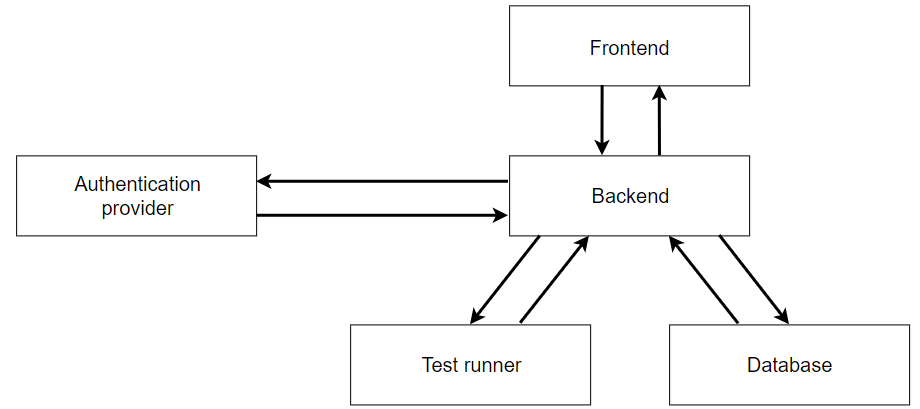
\includegraphics[scale=0.6]{Architecture.PNG}
	\centering
	\caption{The architecture for our web application}
	\label{fig:Architecture}
\end{figure}


\section{Database}
In order to persist data, the backend retrieves and updates data in the database component depicted in figure \ref{fig:Architecture}. This is done through create, read, update and delete operations.
The backend then queries the database and returns the relevant data.

The database component is implemented as a Postgres database. The entities and their relationships contained within the database is shown in figure \ref{fig:Database}. In the figure each box represents an entity-set and attributes for the entities. A diamond represent a relationship between two or more entity-sets.

A dotted line connecting an entity-set to a relationship represent a partial participation of the connected entities and the other participants in the relationship. This means that an entity can exist in the database without participating in the relationship.
A full line connecting an entity-set to a relationship represents total participation of the entity-set symbolizing that an entity must participate in the relationship.
This means that an entity cannot exist in the database without participating in the relationship.
The numbers and letters at the beginning of each relationship line represents the cardinality. A \textit{number} between a relationship and an entity-set represents the number of times an entity can participate in the relationship. Similarly, an \textit{N} represents that entities can participate $0$ or more times.

\begin{figure}[H]
	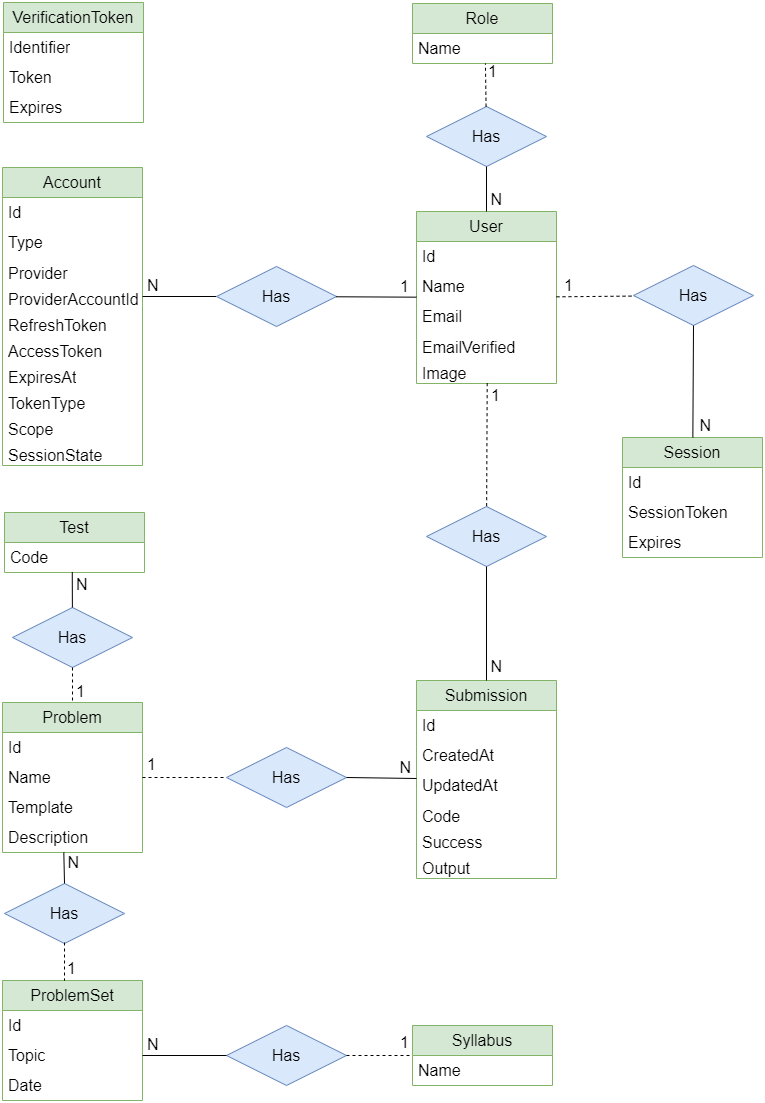
\includegraphics[scale=0.4]{Database.png}
	\centering
	\caption{Entity relationship diagram of the database}
	\label{fig:Database}
\end{figure}

The structure of database can be explained through the two types of users of the system. The lecturer and the student.
In order to support different roles in the system, we have created the entities \textit{Role} and \textit{User}. The \textit{Role} entity has one attribute called \textbf{Name}. This corresponds to the name of the role. The \textit{User} entity has the attributes \textbf{Id}, which is a unique identifier, \textbf{Name}, \textbf{Email}, \textbf{EmailVerifed} which is when the email was verified and an \textbf{Image} attribute which contains the URL for an image of the user. The \textit{User} entity has a many-to-one relationship with the entity \textit{Role}, which means that users can only have one role.

To support a lecturer in creating a syllabus for a semester course we have created the entities \textit{Syllabus}, \textit{Problemset}, \textit{Problem} and \textit{test}. For each entity, a set of attributes have been added to contain the relevant data and relationships between these entities to annotate their relation.
For the \textit{Problem} entity we have added an \textbf{Id} attribute as a unique identifier, a \textbf{Name} attribute, a \textbf{Template} attribute, which contains code that will be automatically included in the editor when starting a problem. This ensures that the functions are included in a module which can later be accessed by \textbf{Hspec}. The final attribute is the \textbf{Description}, which contains the description of the exercise.

The \textit{Test} entity has the attribute \textbf{Code}. This contains the test code that the lecturer has written for a problem. A \textit{Problem} and a \textit{Test} are in a one-to-many relationship with each other, where a \textit{Problem} has many \textit{tests}. This allows a lecturer to define multiple tests for a problem.

The \textit{Problemset} entity corresponds to a course exercise session. It has the attribute \textbf{Id}, which a unique identifier, the attribute \textbf{Topic} which is the topic covered in the session, and lastly a \textbf{Date} which corresponds the when the session occurs. The relationship between the \textit{Problemset} entity and the \textit{Problem} entity is one-to-many, since a problem set has multiple problems. This allows the lecturer to create a set of problems for a course exercise session.

The \textit{Syllabus} entity corresponds to an entire syllabus for a course. The entity only has a \textbf{Name} attribute, which is the name of the course. The \textit{Syllabus} entity has a one-to-many relationship with the \textit{Problemset} entity. This allows the lecturer to create multiple problem sets for a course.

To support a student in submitting solutions to exercises we have created the entity \textit{Submission}. This entity contains the attributes \textbf{Id}, which is a unique identifier, \textbf{CreatedAt} which contains the time for when the submission was first added, \textbf{UpdatedAt} which contains the time when the submission was last updated. It also contains the attributes \textbf{Code}, which contains the code submitted by the student, \textbf{Success} which states whether the submission passed the tests for the problem. Finally it has the attribute \textbf{Output}, which is the standard output from the compiler.
The \textit{Submission} entity is in a many-to-one relationship with the \textit{User} entity, because each user can have many submissions. \textit{Submission} is also in a many-to-one relationship with \textit{Problem}, as a problem can have multiple submissions.

The remaining entities \textit{Account}, \textit{Session} and \textit{VerificationToken} are entities which are required by authentication services and are not developed by us.

\section{Backend System}
The backend component has several responsibilities including routing, page rendering, authentication, role based data access and modification, as well as communication between other components. 
The component enables the creation of accounts for the system by using an authentication provider.
For this project, Google is used as the provider. 
Once a user account is created, it is assigned the default \texttt{Student} role.  
Depending on the account role, the user has different permissions.
A lecturer can create and modify syllabi, problemsets, submissions, problems and tests, while students are only able to view these. Both roles can create submissions.
Data fetching and mutation is facilitated on the Next backend through tRPC and Prisma. In the API routes, user permissions are authorized by getting the requesting user's information and validating it.
Once the backend receives a query or mutation, the given input is validated to ensure that it is of correct structure and type.
If the query or mutation is formatted correctly, and the user has the correct authorization, the Prisma ORM transforms it to database queries, and maps the result to \javascript{} objects.
The backend then sends a response to the user with the requested data.
This system component is implemented using TypeScript and Next.js.

\section{Frontend} \label{sec:architecture-frontend}
The frontend component is the user facing component of our platform.  It contains the user interface for the platform and is the main interface of the system.
The component is designed such that its user interface and functionality depends on the role of the user.
Whenever users make requests to the backend component, the frontend component is responsible for displaying the results of these requests to the user. The data sent is limited to the data the user is authorized for.
The component is also responsible for only providing users with user interface elements they are authorized to view. 
For instance, some edit and delete buttons are available only to lecturers.
The component contains functionality providing users with syntax highlighting using the CodeMirror library. 
It is implemented using TypeScript and React. 

\section{Test Runner}
The test runner component is responsible for determining whether a student's exercise submission solves a problem.
It receives HTTP requests containing Haskell code and an Hspec test, and uses this to stage and perform test execution. 
This is done using the GHC interpreter.
The result of processing the test is then serialized to JSON and sent to the backend component.
The test runner component is implemented as an HTTP server using the axum crate in the Rust programming language.

In the following chapters we will elaborate on the most important components of our system. In these chapters we will give a detailed description of how the components work and their structure.